\documentclass[tikz,border=5pt]{standalone}
\usepackage{amsmath}
\usetikzlibrary{arrows.meta}

\begin{document}
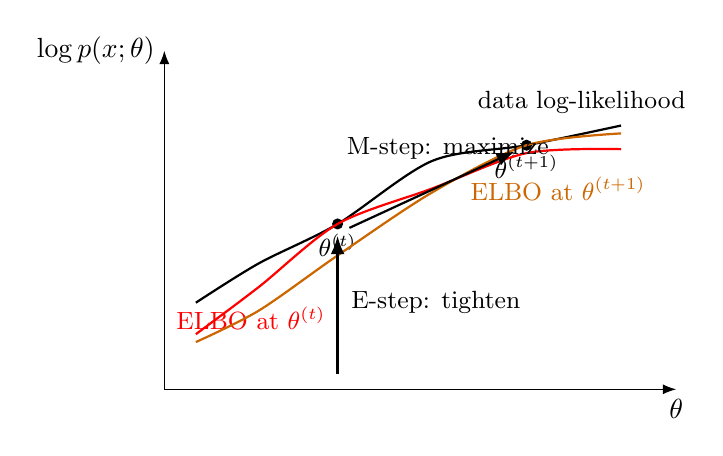
\begin{tikzpicture}[>=Latex,scale=1]

% axes
\draw[->] (0,0) -- (6.5,0) node[below] {$\theta$};
\draw[->] (0,0) -- (0,4.3) node[left] {$\log p(x;\theta)$};

% true log-likelihood curve (white curve in lecture)
\draw[thick] plot[smooth] coordinates {
  (0.4,1.1) (1.2,1.6) (2.2,2.1) (3.4,2.9) (4.6,3.1) (5.8,3.35)
};
\node[black] at (5.3,3.65) {\small data log-likelihood};

% theta_old and theta_new markers
\coordinate (told) at (2.2,2.1);
\coordinate (tnew) at (4.6,3.1);
\fill (told) circle (2pt);
\fill (tnew) circle (2pt);
\node[below] at (told) {\small $\theta^{(t)}$};
\node[below] at (tnew) {\small $\theta^{(t+1)}$};

% ELBO curve touching at theta^{(t)} (red curve)
\draw[thick,red] plot[smooth] coordinates {
  (0.4,0.7) (1.2,1.3) (2.2,2.1) (3.4,2.55) (4.6,3.0) (5.8,3.05)
};
\node[red] at (1.1,0.9) {\small ELBO at $\theta^{(t)}$};

% ELBO curve touching at theta^{(t+1)} (orange curve), indicative of next iteration
\draw[thick,orange!80!black] plot[smooth] coordinates {
  (0.4,0.6) (1.2,1.0) (2.2,1.7) (3.4,2.5) (4.6,3.1) (5.8,3.25)
};
\node[orange!80!black] at (5.0,2.55) {\small ELBO at $\theta^{(t+1)}$};

% arrows for E-step and M-step
\draw[->,thick] (2.2,0.2) -- (2.2,1.95);
\node[right] at (2.25,1.1) {\small E-step: tighten};

\draw[->,thick] (2.35,2.05) -- (4.45,3.02);
\node[above] at (3.6,2.8) {\small M-step: maximize};

\end{tikzpicture}
\end{document}


